\begin{frame}
    \frametitle{Control approach to traffic systems \dots}
    \newcommand*\nodeonecolor{}
    \newcommand*\nodesecondcolor{}
    \only<2>{\renewcommand*\nodeonecolor{blue}}  
    \only<3>{\renewcommand*\nodesecondcolor{blue}}  
    \begin{center}
    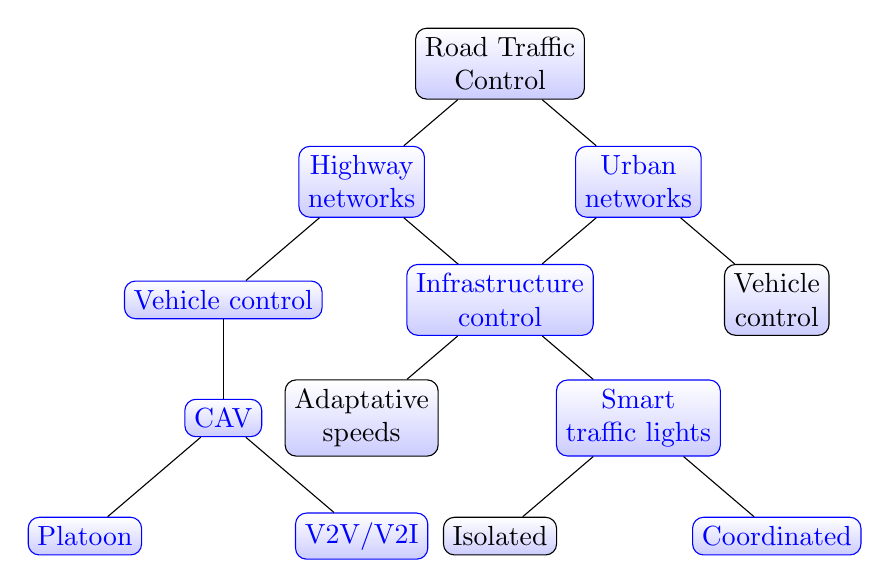
\begin{tikzpicture}[sibling distance=10em,
    every node/.style = {shape=rectangle, rounded corners,
    draw, align=center,
    top color=white, bottom color=blue!20}]]
    \node {Road Traffic\\Control}
    child { 
        node [\nodesecondcolor]{Highway\\networks}
        child{
            node [\nodesecondcolor]{Vehicle control} 
            child{
                node [\nodesecondcolor]{CAV}
                child{
                    node [\nodesecondcolor]{Platoon}
                }
                child{
                    node [\nodesecondcolor]{V2V/V2I}
                }
            }
        } 
        child{
            node {Space control}
        }
    }
    child { 
        node [\nodeonecolor]{Urban\\networks}
        child { 
            node [\nodeonecolor]{Infrastructure\\control}
            child{ 
                node {Adaptative\\speeds} 
            }
        child{ 
            node [\nodeonecolor]{Smart\\ traffic lights}
            child { 
                node {Isolated} 
            }
            child { 
                node [\nodeonecolor]{Coordinated} 
                } 
            } 
        }
        child { 
            node {Vehicle\\control}
        } 
    };
    \end{tikzpicture}
    \end{center}
\end{frame}
